\documentclass{report}
    \title{50004 - Operating Systems - Lecture 2}
    \author{Oliver Killane}
    \date{15/10/21}

%===========================COMMON FORMAT & COMMANDS===========================
% This file contains commands and format to be used by every module, and is 
% included in all files.
%===============================================================================

%====================================IMPORTS====================================
\usepackage[a4paper, total={6in, 8in}]{geometry}
\usepackage{graphicx, amssymb, amsfonts, amsmath, xcolor, listings, tcolorbox, multirow, hyperref}
%===============================================================================

%====================================IMAGES=====================================
\graphicspath{{image/}}

% \centerimage{options}{image}
\newcommand{\centerimage}[2]{\begin{center}
    \includegraphics[#1]{#2}
\end{center}}
%===============================================================================

%==============================SYNTAX HIGHLIGHTING==============================
\newcommand{\fun}[1]{\textcolor{blue}{\textbf{#1}}}
\newcommand{\file}[1]{\textcolor{green}{\textbf{#1}}}
\newcommand{\struct}[1]{\textcolor{orange}{\textbf{#1}}}
\newcommand{\var}[1]{\textcolor{purple}{\textbf{#1}}}
\newcommand{\const}[1]{\textcolor{red}{\textbf{#1}}}
%===============================================================================

%=================================CODE LISTINGS=================================
\definecolor{codebackdrop}{gray}{0.9}
\definecolor{commentgreen}{rgb}{0,0.6,0}
\lstset{
    inputpath=code, 
    commentstyle=\color{commentgreen},
    keywordstyle=\color{blue}, 
    backgroundcolor=\color{codebackdrop}, 
    basicstyle=\footnotesize,
    frame=single,
    numbers=left,
    stepnumber=1,
    showstringspaces=false,
    breaklines=true,
    postbreak=\mbox{\textcolor{red}{$\hookrightarrow$}\space}
}

% Create a code listing for a single line
% \codeline{language}{line}{file}
\newcommand{\codeline}[3]{\lstinputlisting[language=#1, firstline = #2, lastline = #2]{#3}}

% Create a code listing for multiple lines
% \codeline{language}{start}{end}{file}
\newcommand{\codelines}[4]{\lstinputlisting[language=#1, firstline = #2, lastline = #3]{#4}}


% Create a code listing for a given language & file
% \codelist{language}{file}
\newcommand{\codelist}[2]{\lstinputlisting[language=#1]{#2}}
%===============================================================================

%================================TEXT STRUCTURES================================
% Marka a word as bold
% \keyword{important word}
\newcommand{\keyword}[1]{\textbf{#1}}

% Creates a section in italics
% \question{question in italics}
\newcommand{\question}[1]{\textit{#1} \\ }

% Creates a box with title for side notes.
% \sidenote{title}{contents}
\newcommand{\sidenote}[2]{\begin{tcolorbox}[title=#1]#2\end{tcolorbox}}

\newcommand{\termdef}[2]{\begin{tcolorbox}[title=Definition: #1, colframe = blue]#2\end{tcolorbox}}

% Creates an item in an itemize or enumerate, with a paragraph after
% \begin{itemize}
%     \bullpara{title}{contents}
% \end{itemize}
\newcommand{\bullpara}[2]{\item \textbf{#1} \ #2}

% Creates a compact list (very small gaps between items)
% \compitem{
%     \item item 1
%     \item item 2
%     \item ...
% }
\newcommand{\compitem}[1]{\begin{itemize}\setlength\itemsep{-0.5em}#1\end{itemize}}
\newcommand{\compenum}[1]{\begin{enumerate}\setlength\itemsep{-0.5em}#1\end{enumerate}}

% Creates a link to the lecture for use at the start of the notes document
\newcommand{\lectlink}[1]{\sidenote{Lecture Recording}{
    Lecture recording is available \href{#1}{here}
}}
%===============================================================================

%================================STYLIZED PROOFS================================
%For ease in writing stylized proofs with numbers
\newcommand{\stepno}[1]{\textcolor{red}{\textbf{#1}}}

\newenvironment{proof}
{\begin{center}\begin{tabular}{r l l }}
{\end{tabular}\end{center}}

%\proofstep{step}{workings}{description}
\newcommand{\proofstep}[3]{\stepno{(#1)} & #2 & #3 \\}
%===============================================================================

%==============================UNFINISHED SECTION===============================
\newcommand{\unfinished}{\begin{huge} \textcolor{red}{\textbf{UNFINISHED!!!}} \end{huge}}
%===============================================================================

%==============================THREAD HIGHLIGHTING==============================
\newcommand{\threada}[1]{\textcolor{green}{\textbf{#1}}}
\newcommand{\threadb}[1]{\textcolor{red}{\textbf{#1}}}
%===============================================================================

%============================DISPLAYING THREAD CODE=============================
\newcommand{\threadlist}[3]{
    \codelist{#1}{#2 init.#3}
    \begin{minipage}[t]{0.45\textwidth}
        \codelist{#1}{#2 A.#3}
    \end{minipage}
    \hfill
    \begin{minipage}[t]{0.45\textwidth}
        \codelist{#1}{#2 B.#3}
    \end{minipage}
}
%===============================================================================


\begin{document}
    \maketitle
    \sidenote{Lecture Recording}{
        Lecture recording is available \href{https://imperial.cloud.panopto.eu/Panopto/Pages/Viewer.aspx?id=2c738232-4a28-4565-8251-adc100a6a1ad}{here}
    }

    \section*{Processes}
        Processes are one of the oldest abstractions in computing, holding an instance of a running program.
        \begin{center}
            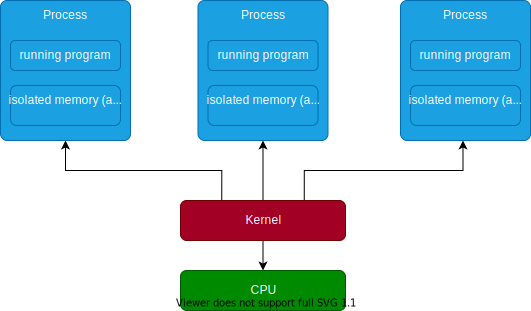
\includegraphics[width=0.5\textwidth]{process.png}
        \end{center}
        The process abstraction can allow and OS to run programs simultaneously, even on only one CPU core.
        \\
        \\ Each process runs on a isolated \keyword{virtual CPU}, to achieve this the CPU resources of the system are multiplexed \& managed by the OS.
        \subsubsection*{Why Have Processes?}
            \begin{itemize}
                \bullpara{Provide Concurrency}{
                    To ensure real concurrency works properly (programs running on multiple CPU cores).
                    \\
                    \\ And to manage a single CPU core so that multiple processes can appear to run simultaneously, each process running independently.
                }
                \bullpara{Provide Isolation}{
                    Each process has its own address space, and does not need to consider other unrelated processes in order to run correctly.
                }
                \bullpara{Simplify Programming}{
                    Applications can be easily developed to run without needing to consider how resources will be managed, or what other applications may be running. Programs can be written as if they will be run without any other programs running.
                }
                \bullpara{Better Resource Utilisation}{
                    Different processes require different resources. Hence we can more effectively increase utilisation \& performance with multiple processes even on a single CPU core.
                    \\
                    \\ For example a program may need to wait on I/O, rather than leaving this process idling while waiting, other programs can be scheduled to make use of resources during thwe wait.
                }
            \end{itemize}
            \sidenote{Address Space}{
                A process' address space is a contiguous region of memory allocated to a process by the operating system for use in storing data.
                \\
                \\ A process accesses this region using \keyword{virtual addresses} indexed from $0$.
                \begin{center}
                    \includegraphics[width=\textwidth]{address space.png}
                \end{center}
            }
    \section*{Multitasking}
        \subsubsection*{Time Slicing}
            Processes are given a set \keyword{time slice} to run on the CPU, before a \keyword{context-switch} is done to another process.
            \\
            \\ By switching between processes very quickly, the illusion of concurrency can be achieved on a single CPU core.
            \sidenote{Context Switch}{
                A context switch is where the CPU switches from the running one process/thread, to running another.
                \\
                \\ To achieve this the switch must:
                \begin{enumerate}
                    \item store the current state (Registers such as the stack pointer) such that it can be resumed later.
                    \item Load the previously stored state of another thread/process (registers such as stack pointer)
                    \item Resume processing the current thread (now switched)
                \end{enumerate}
                This can occur due to an interrupt (e.g timer interrupts for a time slice strategy, accessing disk and other I/O etc) or in some systems when moving between \keyword{user mode} and \keyword{kernel mode} tasks.
                \\
                \\ Context switches are an essential feature of any multitasking operating system. Too many context switches can have a negative impact on performance.
            }
        \subsubsection*{Pesudo Concurrency}
            Single processor, processes are interleaved to give the illusion of concurrency.
            \begin{center}
                \includegraphics[width=\textwidth]{pesudo concurrency.png}
            \end{center}
        \subsubsection*{Real Concurrency}
            Several processors, running threads in parallel. Pesudo concurrency can also be employed (e.g in the diagram, 2 CPUs, 4 processes).
            \begin{center}
                \includegraphics[width=\textwidth]{real concurrency.png}
            \end{center}
        \subsubsection*{Fairness}
            When implementing a scheduler to determine when threads run we must consider how much time is allocated to each.
            \\
            \\ When one application is using too much CPU time, other processes may lagg (latency) and perform badly. Likewise if a process is not allocated sufficient resources.
        \subsubsection*{Higher CPU Utilisation}
            We can switch to other threads when the current thread is waiting, instead of idling. This is beneficial so long as the context switch overhead is smaller than the utilisation that would've been lost to waiting.
            \begin{center}
                \includegraphics[width=\textwidth]{IO waiting.png}
            \end{center}
            We can compute an estimate for CPU utilisation on a uniprocessor:
            \[\begin{matrix}
                n & = & \text{total number of processes} \\
                p & = & \text{Fraction of time a process is waiting for I/O} \\
            \end{matrix}\]
            \[Prob(\text{all waiting for I/O}) = p^n\]
            \[CPU utilisation = 1- p^n\]
        \subsection*{Process Control Block}
            A \keyword{Process Control Block} contains a process's information:
            \begin{itemize}
                \bullpara{Process Identification}{
                    The process's unique ID, its group, parent etc. Used to identify what resources (e.g perhiperals) the process is using.
                }
                \bullpara{Process State Data}{
                    Values of saved registers (when suspended), such as the stack pointer, page table register etc.
                }
                \bullpara{Process Control Information}{
                    \begin{itemize}
                        \item Scheduling state (e.g ready, suspended, blocked)
                        \item Priority values (for priority scheduling)
                        \item Related process IDs (e.g parent)
                        \item \keyword{IPC} information (flags, signals and messages associated with communication among independent processes)
                        \item Process privileges (e.g file access, peripheral access)
                        \item Usage Statistics such as recent CPU time, used for scheduler priority calculations.
                    \end{itemize}
                }
                \bullpara{File Management Info}{
                    Root directory, working directory and open file descriptors.
                }
            \end{itemize}
        \subsubsection*{Context Switch Expense}
            Context switches are expensive, and have considerable overhead, so we must avoid them if possible.
            \\
            \\ \textbf{Direct Cost:} save/restore process state.
            \\ \textbf{Indirect Cost:} pertubation of memory caches, TLB
            \sidenote{Transaltion Lookaside Buffers}{
                A cache storing recent translations of virtual addresses to physical addresses (used as user programs use virtual addresses to access their own address space).
                \\
                \\ It is a hardware feature that is part of a memory-management unit (MMU) and can reside between the CPU \& CPU cahce, or between CPU cahce and the main memory.
                \\
                \\ During a context switch these are typically flushed.
            }
    \section*{Process Lifecycle}
        \subsubsection*{Process Creation}
            \begin{itemize}
                \item System initialisation (start services, e.g file system)
                \item User request (run a program)
                \item Process Request (process makes a system call to start a new process)
            \end{itemize}
            \sidenote{Daemon}{
                A background process, typically does not interact directly with users, e.g sshd (linux) listens for connections from clients, and forks a new daemon to manage each new connection.
            }
        \subsubsection*{Destruction}
            \begin{itemize}
                \bullpara{Completion}{
                    \\ Once at the end of execution body (main function returns), the process ends.
                }
                \bullpara{System Call}{
                    \begin{tabular}{r l}
                        \textbf{UNIX}: & exit() \\
                        \textbf{Windows}: &  ExitProcess()
                    \end{tabular}
                }
                \bullpara{Abnormal Exit}{
                    \\ The process runs into an error or unhandled exception, and is forced to stop.
                }
                \bullpara{Aborted}{
                    \\ Process stops because another process forces its execution to end. e.g parent process (terminal) forces child (program) to end.
                }
                \bullpara{Never}{
                    \\ Some never terminate, many daemons need to be running at all timnes to ensure the OS or some crtitcal application being run functions as it should.
                }
            \end{itemize}
        \subsubsection*{Process Hierarchies}
            \keyword{UNIX} has a strict tree of processes.
            \begin{center}
                \includegraphics[width=\textwidth]{unix processes.png}
            \end{center}
            \begin{itemize}
                \item On boot, \keyword{init} is created, this is the root of the process hierarchy tree (\keyword{process group}).
                \item Reads a file to determine how many processes need to be run, forks off one terminal per terminal.
                \item Each terminal waits for a user to login.
                \item On successful login, the login process executes a shell to accept commands which may in turn spawn more processes.
            \end{itemize}
            \keyword{Windows} has no such enforced hierarchy, upon spawning a process the parent is given a token/handle to control the child. This token can be transferred to other processes.
    \section*{UNIX Processes}
        \subsubsection*{fork}
            \lstinputlisting[language=C,firstline=1,lastline=1]{process declarations.c}
            Fork creates an identical copy of the process, the child process iherits resources of the parent process and is run concurrently.
            \\\begin{tabular}{r l}
                \textbf{Return} & \textbf{Reason} \\
                $0$ & You are the child \\
                $-1$ & fork failed (out of memory, max process limit reached, etc) \\
                $n$ & You are the parent, pid $n$ is the child. \\
            \end{tabular}
            \lstinputlisting[language=C]{fork.c}

        \subsubsection*{Executing Processes}
            \lstinputlisting[language=C,firstline=2,lastline=2]{process declarations.c}
            Changes the process image and runs new process.
            Arguments:
            \begin{itemize}
                \bullpara{path}{Full pathname to program to run}
                \bullpara{argv}{arguments to pass to main}
                \bullpara{envp}{environment variables (e.g \const{\$PATH)} \const{\$HOME}}
            \end{itemize}
            There are many useful wrappers to make calls easier/cleaner such as; \function{execl}, \function{execle}, \function{execvp}, \function{execv}...
        \subsubsection*{Waiting for Process Termination}
            \lstinputlisting[language=C,firstline=3,lastline=3]{process declarations.c}
            Suspends the current process until the process \keyword{PID} has terminated.
            \\ \begin{tabular}{r l}
                \keyword{PID} & \textbf{Result} \\
                $-1$ & Wait for any child \\
                $0$ & Wait for any child in the same \keyword{process group} as the caller \\
                $-gid$ & Wait for any child with \keyword{process group} $gid$ \\
                $pid$ & wait for process $pid$ \\
            \end{tabular}
            \\
            \\ \sidenote{Process Group}{
                A collections of processes, typically used for signal distribution. 
                \\
                \\ When a \keyword{process group} is signalled, every contained process receives the signal, and can further direct it to other process groups.
                \\
                \\ For example in the terminal, keyboard input can be sent to the terminal application, and the propagated to all running programs of that terminal instance.
            }
            Return value is as follows:
            \\ \begin{tabular}{r l}
                \textbf{Value} & \textbf{Result} \\
                $0$ & if \const{WNOHANG} is in set options (call should not block) \\
                $-1$ & if an error occured, \structure{errorno} set to indicate error \\
                $pid$ & \keyword{PID} of process that terminated. \\
            \end{tabular}

            \lstinputlisting[language=C]{command interpreter.c}
        \subsubsection*{Process Termination}
            \lstinputlisting[language=C,firstline=4,lastline=4]{process declarations.c}
            Terminates the process (called implicitly when execution finishes), returns exit status to the parent process.
            \lstinputlisting[language=C,firstline=5,lastline=5]{process declarations.c}
            Kill process using \keyword{PID}, by sending a signal to the process.
            
        \subsubsection*{UNIX Philosophy}
            \keyword{UNIX} places value on building basic blocks to be combined into more complex programs, \function{fork} is an example of this, while \function{execve} could be used to replicate fork, it would be far more complex.
            \\
            \\ Windows does not follow this design philosophy, \function{createProcess} is the equivalent if \function{fork} and \function{execve}. It has 10 parameters for:
            \begin{itemize}
                \item program to execute
                \item parameters
                \item security attributes
                \item meta data for files
                \item priority
                \item pointer to info regarding new process
                \item and more!
            \end{itemize}
            \lstinputlisting[language=C,firstline=6,lastline=19]{process declarations.c}
    \section*{Process Communication}
        \subsubsection*{UNIX Signals}
            A limited form of \keyword{IPC} that works similarly to handler interrupts. A process can send a signal to another process if it has permission (same user for receiver or elevated privileges), the kernel can send a signal to any thread.
            \\
            \\ Signals can be triggered by:
            \begin{itemize}
                \bullpara{Exceptions}{(e.g Zero division error (SIGFPE) or segfault (SIGSEGV))}
                \bullpara{Events}{e.g Kernel notifies a process if it writes to a closed pipe (SIGPIPE), or input (keyboard interrupt $\to$ SIGINT)}
                \bullpara{Programatically}{Using the \function{kill} system call.}
            \end{itemize}
            Common Signals are as follows
            \begin{center}
                \begin{tabular}{r l}
                    \textbf{Signal} & \textbf{Description} \\
                    SIGINT & Interrupt from keyboard \\
                    SIGABRT & Abort signal from abort \\
                    SIGFPE & Floating point exception \\
                    SIGKILL & Kill signal \\
                    SIGSEGV & Invalid memory reference \\
                    SIGPIPE & Broken pipe: write to pipe with no readers \\
                    SIGALRM & Timer signal from alarm \\
                    SIGTERM & Termination signal \\
                \end{tabular}
            \end{center}
        \subsubsection*{Signal Handlers}
            The default action for most signals is to terminate the process, however processes can register their own signal handlers.
            \lstinputlisting[language=C]{signal handler.c}
        
        \subsubsection*{UNIX Pipes}
            A pipe connects the standard output of one process to the standard input of another.
            \begin{center}
                \includegraphics[width=0.7\textwidth]{pipe.png}
            \end{center}
            \lstinputlisting[language=C, firstline=17, lastline=17]{process declarations.c}
            \begin{tabular}{r l}
                fd[0] & read end (closed by sender) \\
                fd[1] & write end (closed by receiver) \\
            \end{tabular}
            \\ When the receiver reads from an empty pipe, it is blocked until more data is written.
            \\ When the sender writes to a full pipe, it is blocked until data is read and removed from the pipe.
            \lstinputlisting[language=C]{pipe.c}

        \subsubsection*{UNIX Named Pipes}
            Persistent pipes outlive the processes which create them and are stored in the file system.
            \lstinputlisting[language=Bash]{persistent pipe.sh}
\end{document}
